\documentclass{article}
\usepackage[utf8]{inputenc}
\usepackage{graphicx}
\title{CARA MEMBUAT APLIKASI PENDATAAN GAJI PEGAWAI PADA APEC}
\author{Gany Berdu Sura - 1184008 }
\date{Desember 2019}

\begin{document}

\maketitle
\section{Pembuatan Table sebelum aplikasi}
\begin{enumerate}
    \item hal pertama yang harus dilakukan adalah membuat tabel terlebih dahulu atau data-data oegawai dan gaji pegawai.
    bukalah oracle apec dan masuk dengan menggunakan akun yang telah terdaftar seperti dibawah ini, jangan lupa memasukan workspace yang telah dibuat sebelumnya.
    \begin{center}
    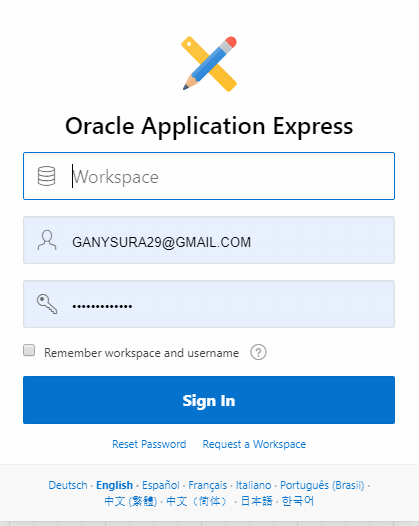
\includegraphics[width=.6\textwidth]{gambar/satu.PNG}
    \end{center}
    \item kemudian pilih SQL Workshop dan pilih SQL Commands
    \begin{center}
    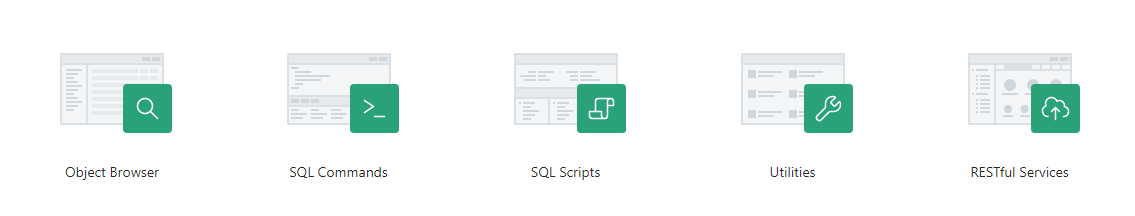
\includegraphics[width=.6\textwidth]{gambar/dua.PNG}
    \end{center}
    \item setelah terbuka, ketikan query perintah membuat table dengan perintah create table yang berarti menciptakan table baru dengan values yang kita tentukan.kemudian setelah terbuka ganti nama tabel dan sesuaikan dengan tabel setiap data, kemudian create. pertama tama buatlah table Pegawai dengan isinya seperti NIP(sebagai PK), nama pegawai, dengan gaji ke yang dimana values gaji ke ini akan di masukan perintah trigger agar akan mendapatkan penambahan data
    \begin{center}
    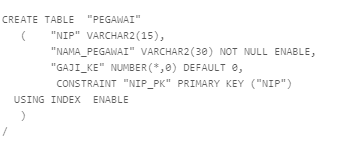
\includegraphics[width=.6\textwidth]{gambar/tigaa.PNG}
    \end{center}
    \item kemudian setelah itu Create table alamat dengan values seperti dibawah ini dan jadikan kode kota sebagai PK"primary key"
    \begin{center}
    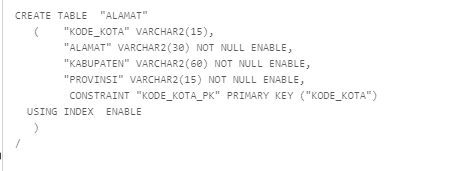
\includegraphics[width=.6\textwidth]{gambar/lima.PNG}
    \end{center}
    \item selanjutnya buat table ketiga dimana pada table ini dijadikan sebagi table pokok dikarenanakn table ini akan menampung foreigen key dari kedua table diatas, yaitu table Gaji dengan values seperti dibawah ini dengan menjadikan NIP sebagai Primary key dan kode kota pada alamat dijadikan sebagai Foreigen key dan NIP pada pegawai dijadikan sebagai foreigen key pada tabel ini agar terjadi korelasi dan hubungan antar table.
    \begin{center}
    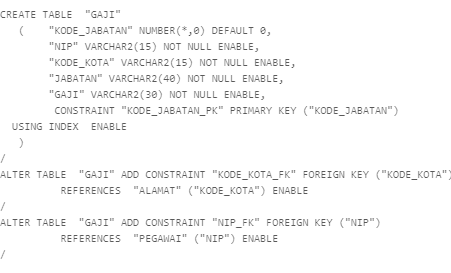
\includegraphics[width=.6\textwidth]{gambar/empat.PNG}
    \end{center}
    \item setelah semua tabel terbuat, cek kembali pada table yang terbuat, jika primary key hingga foreigen key telah terdapat dalam table selanjutnya yang kita buat adalah membuat trigger.
    sedikit penjelasan mengenai trigger, jadi trigger dalam database adalah kode prosedural yang secara otomatis dijalankan untuk menanggapi perubahan tertentu pada table tertentu atau tampilan dalam database. Idealnya, Trigger harus dipertimbangkan ketika kode ini digunakan untuk mengotomatisasi perubahan yang spesifik untuk database atau pengelolaan data. Log audit adalah contoh penerapan dari Trigger.
    setelah mengetahui arti da fungsi trigger maka selanjutnya adalah membuat trigger pada SQL Command dengan query seperti dibawah ini.
    \begin{center}
    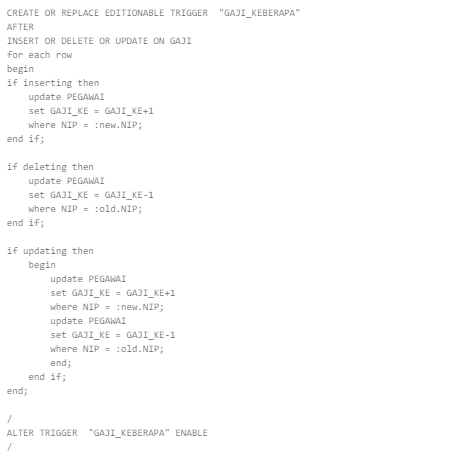
\includegraphics[width=.6\textwidth]{gambar/enam.PNG}
    \end{center}
    maksud dari trigger diatas adalah jika terjadi penambahan gaji pada salah satu pegawai maka kita bisa mengetahui sudah berapa kali si pegawai itu menerima gaji dalam setahun. 
    bisa dilihat pada tabel yang sudah jadi seperti dibawah ini.
     \begin{center}
    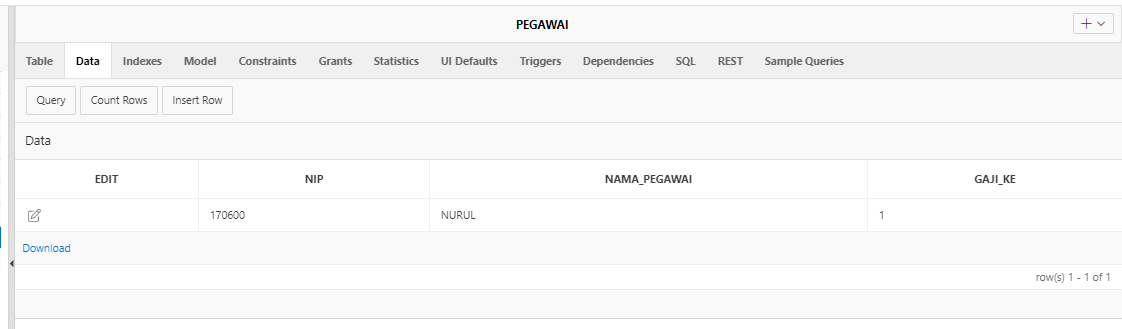
\includegraphics[width=.6\textwidth]{gambar/sembilan.PNG}
    \end{center}
    ssebelum mengetahui hal tersebut, masukan query insert , dimana query ini berfungsi menambahkan data agar bisa dilihat penambahan data yang tertambah.
     \begin{center}
    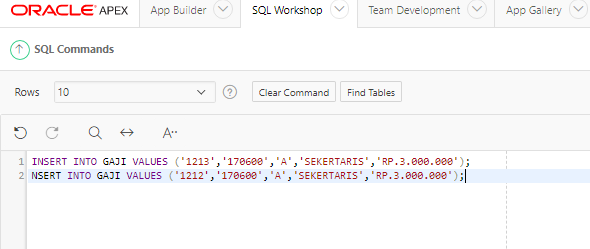
\includegraphics[width=.6\textwidth]{gambar/delapan.PNG}
    \end{center}
    awalnya si pegawai atas nama nurul baru 1 kali mendapat gaji sehingga tercantum 1 kali , namun setelha menggunakan querry trigger diatas maka kita akan mengetahui pertambahan berapa kali si pegawai atas nama nurul bertambah, bisa dilihat pada tabel dibawah ini.
     \begin{center}
    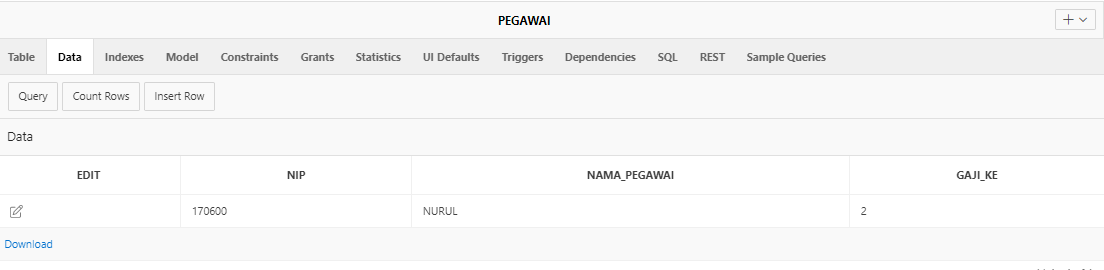
\includegraphics[width=.6\textwidth]{gambar/sepuluh.PNG}
    \end{center}
    jika terjadi perjumlahan gaji berarti triggernya berhasil
    \item setelah itu, kita bisa menggunakan perintah atau query lain yaitu dengan CREATE VIEW, dimana perintah ini berfungsi menampilkan table yang isinya diambil dari tabel tabel yang sudah ada.
    \begin{center}
    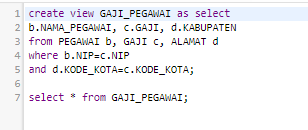
\includegraphics[width=.6\textwidth]{gambar/tujuh'.PNG}
    \end{center}
\section{Pembuatan aplikasi}
    \item buka Appec atau mysql seperti biasa, buka app builder dan klik CREATE
    \begin{center}
    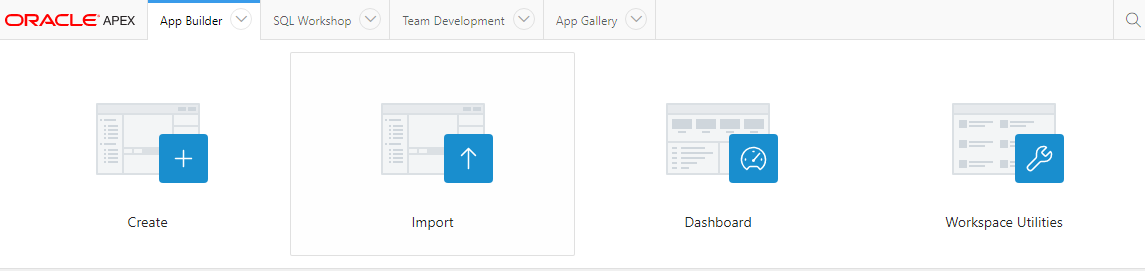
\includegraphics[width=.6\textwidth]{gambar/1.PNG}
    \end{center}
    \item setelah itu pilih NEW APPLICATION
    \begin{center}
    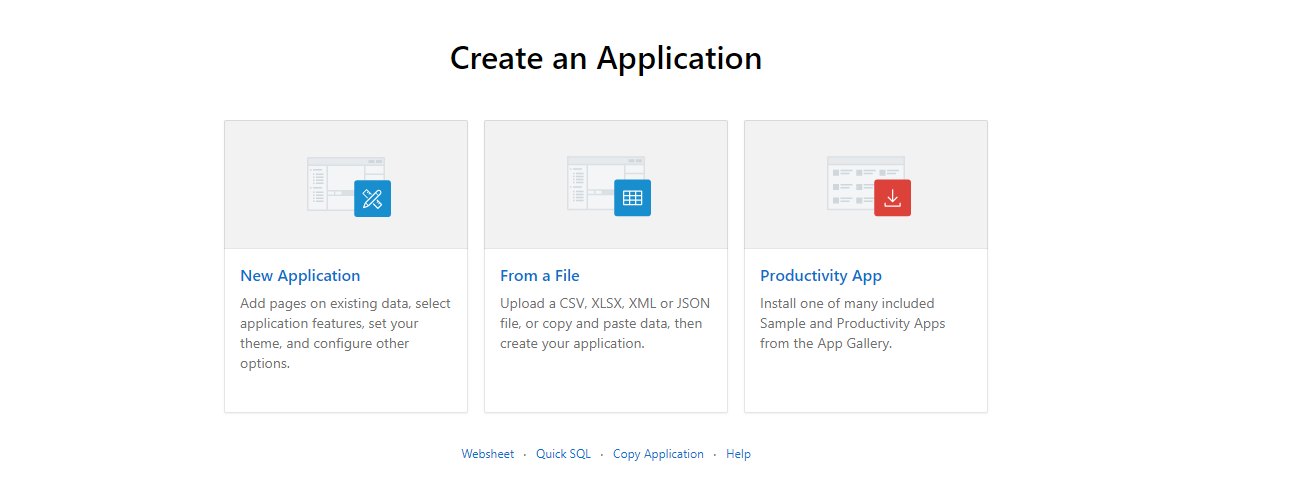
\includegraphics[width=.6\textwidth]{gambar/2.PNG}
    \end{center}
    \item setelah terbuka, buatlah nama aplikasi yang di inginkan
    \begin{center}
    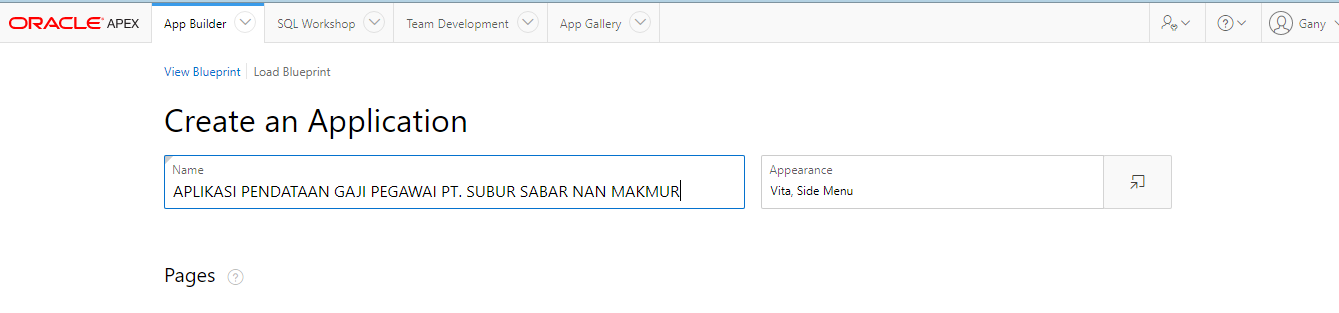
\includegraphics[width=.6\textwidth]{gambar/3.PNG}
    \end{center}
    \item pilih ADD PAGE
    \begin{center}
    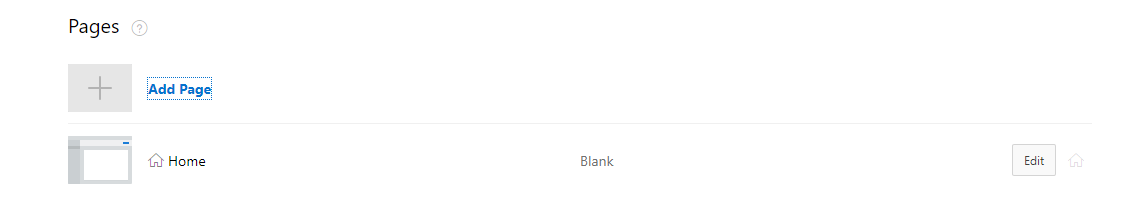
\includegraphics[width=.6\textwidth]{gambar/4.PNG}
    \end{center}
    \item kemudian pilih interactiv report
    \begin{center}
    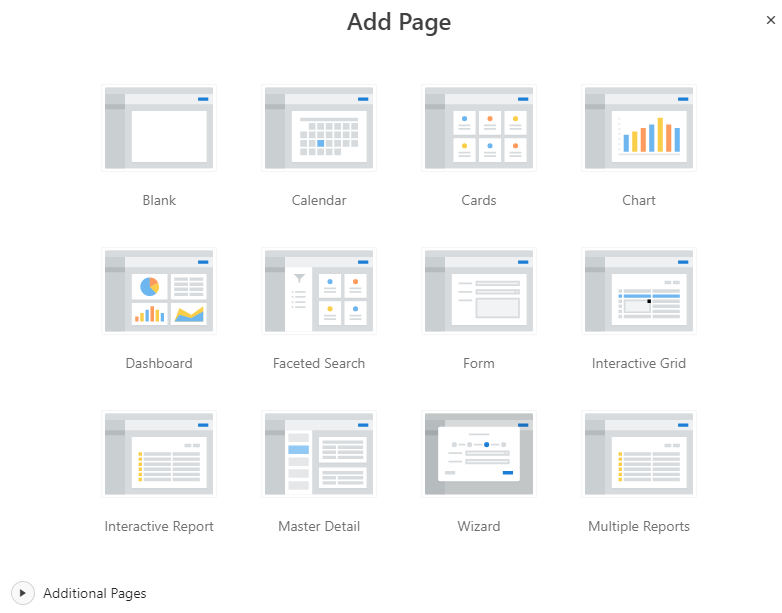
\includegraphics[width=.6\textwidth]{gambar/5.PNG}
    \end{center}
    \item kemudian ganti page name dan nama tabel yang dipilih, lakukan untuk ketiga tabel yang dibuat, jangan lupa mencentang bagian include form dan add pages
    \begin{center}
    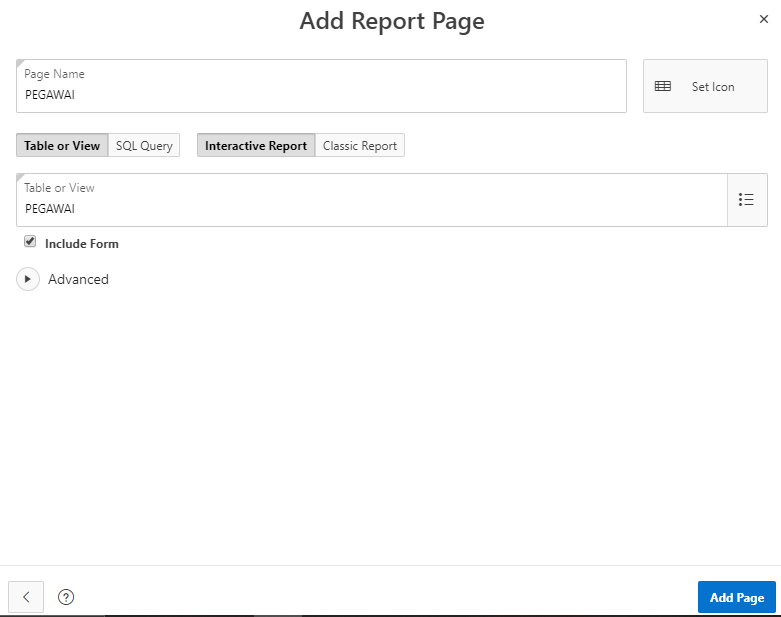
\includegraphics[width=.6\textwidth]{gambar/yaya.PNG}
    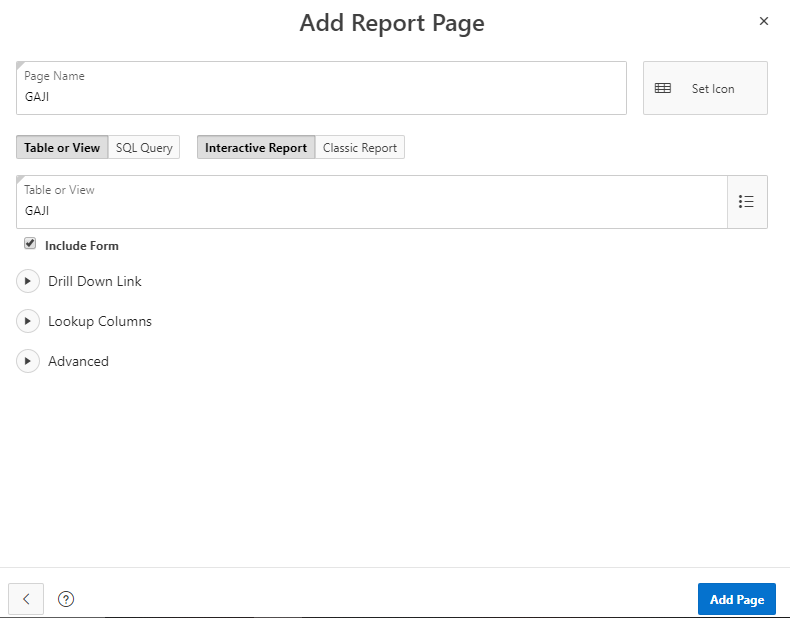
\includegraphics[width=.6\textwidth]{gambar/yiyi.PNG}
    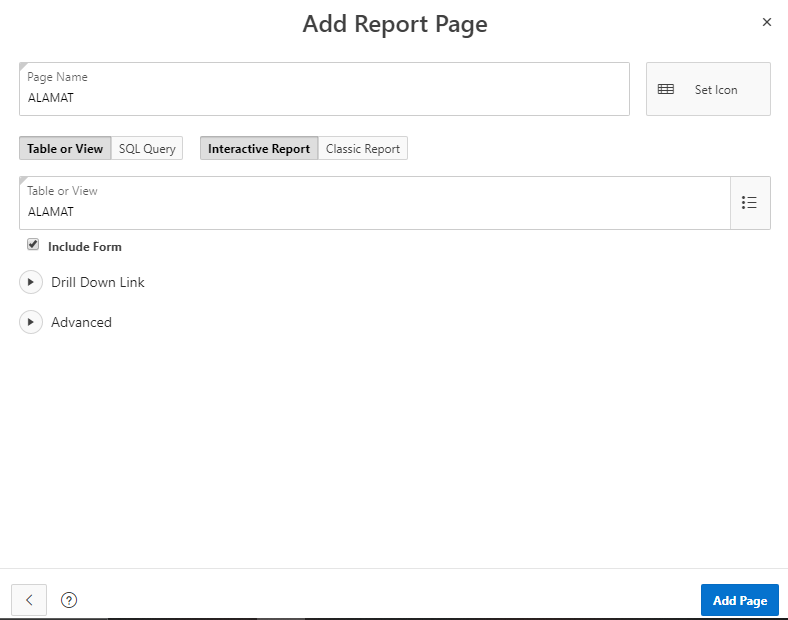
\includegraphics[width=.6\textwidth]{gambar/yuyu.PNG}
    \end{center}
    \item setelah itu, ceklish bagian check all dan create application dan kemudian tunggu
    \begin{center}
    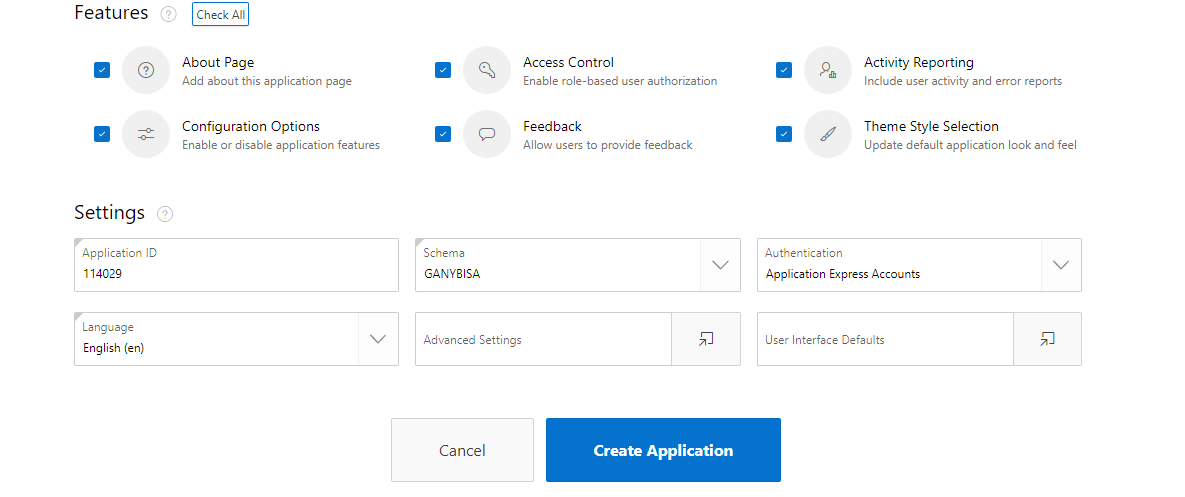
\includegraphics[width=.6\textwidth]{gambar/7.PNG}
    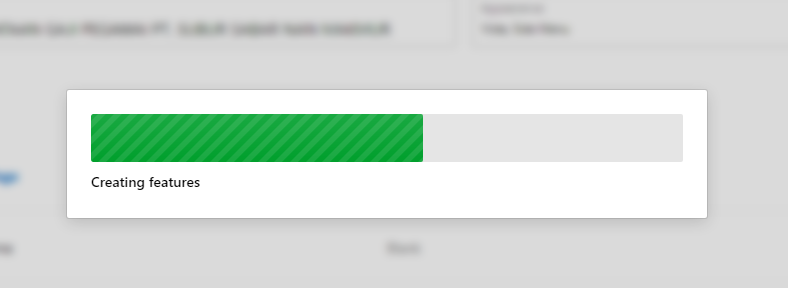
\includegraphics[width=.6\textwidth]{gambar/8.PNG}
    \end{center}
    \item setelah selesai, klik RUN 
    \begin{center}
    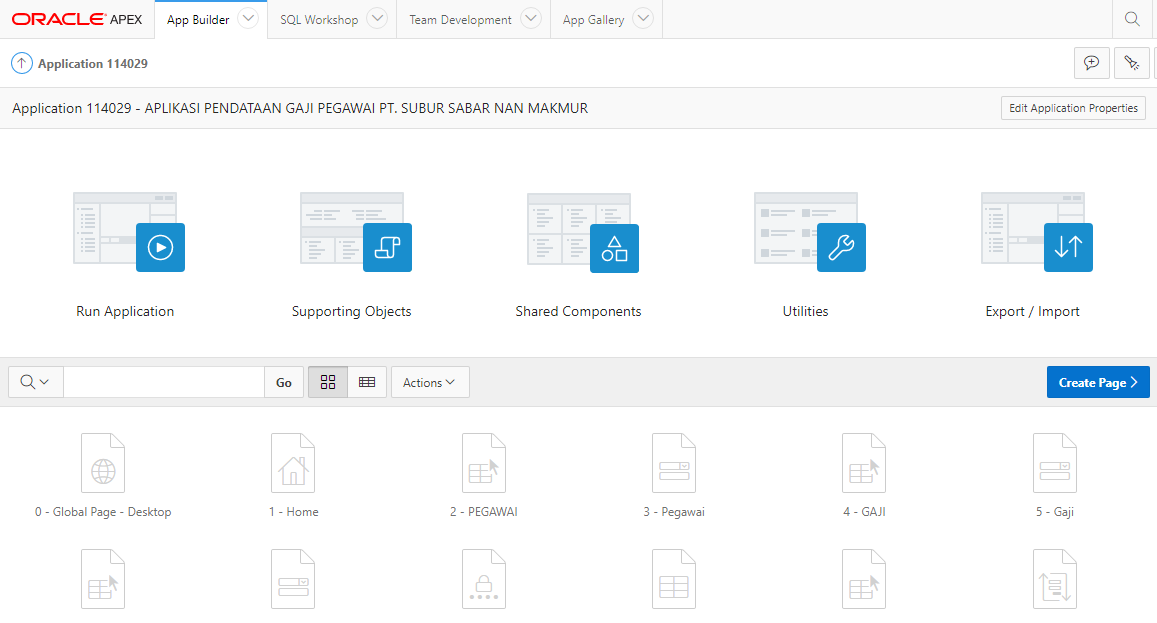
\includegraphics[width=.6\textwidth]{gambar/9.PNG}
    \end{center}
    \item AKUN APEC
    https://apex.oracle.com/pls/apex/f?p=114029:LOGIN_DESKTOP:115053873105116:::::
    EMAIL : GANYSURA29@GMAIL.COM
    SANDI : tujuhbelasjuni2000
\end{enumerate}

\end{document}
